\documentclass[tikz,border=5mm]{standalone}
\usepackage{tikz}
\usetikzlibrary{arrows.meta, positioning, shapes.geometric, calc, backgrounds, fit, matrix, patterns, decorations.pathmorphing, shadows}

% --- COLOR DEFINITIONS ---
\definecolor{Garnet}{HTML}{73000A}
\definecolor{CSecondaryRed}{HTML}{CC2E40}
\definecolor{CBlue}{HTML}{466A9F}
\definecolor{CDark}{HTML}{1F414D}
\definecolor{COlive}{HTML}{65780B}
\definecolor{CLime}{HTML}{CED318}
\definecolor{CGold}{HTML}{A49137}
\definecolor{CGrayLight}{HTML}{E5E5E5}
\definecolor{CGrayDark}{HTML}{555555}
\definecolor{CWhite}{HTML}{FFFFFF}
\definecolor{CBlack}{HTML}{000000}

\begin{document}

\begin{tikzpicture}
    \matrix[column sep=1cm] {
        \node (cam1) {
            \begin{tikzpicture}
                \draw[thick, fill=CWhite] (-0.5,0) rectangle (0.5, 0.8);
                \draw[thick, fill=CWhite] (0, 0.8) circle (0.5);
                \draw[fill=black] (0, 0.8) circle (0.2);
                \node at (0, -0.5) {\textbf{Cam 1 (Fixed)}};
                \draw[<->] (-0.6, 0) -- (-0.6, 1.3) node[midway, left] {H};
            \end{tikzpicture}
        }; &
        \node (cam2) {
            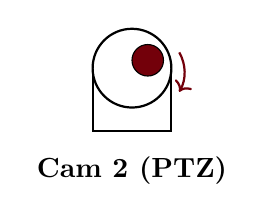
\begin{tikzpicture}
                \draw[thick, fill=CWhite] (-0.5,0) rectangle (0.5, 0.8);
                \draw[thick, fill=CWhite] (0, 0.8) circle (0.5);
                \draw[fill=Garnet] (0.2, 0.9) circle (0.2);
                \draw[->, thick, Garnet] (0.6, 1.0) arc (30:-30:0.5);
                \node at (0, -0.5) {\textbf{Cam 2 (PTZ)}};
            \end{tikzpicture}
        }; \\
    };
    \draw[thick] (cam1.south west) ++(-0.2, 0.2) -- (cam2.south east) ++(0.2, 0.2) node[right] {Mounting Rail};
\end{tikzpicture}

\end{document}
